\section{Separation von Amplitude und Phase}
\label{complex:separate}
\rhead{Separation Amplitude / Phase}

Bei den bisherigen Beispielen mit dem Haar- und Gabor-Wavelet haben wir gesehen, dass die Wahl des Wavelets das erhaltene Bild stark beeinflusst.
Beiden Beispielen gemein war jedoch, dass die Schwingung des Signals in der Amplitude erhalten blieb.
Das Skalarprodukt zwischen Signal und Wavelet ist also abhängig von der Phase maximal, null, minimal, null, maximal, \textellipsis

Diese Oszillation in der Amplitude ist unschön, da sich etwa $a_\text{max}(b)$ so nicht richtig bestimmen lässt.
Dieser Abschnitt dreht sich um die Lösung dieses Problems.
Ziel ist es, am Ende einen Operator $\Ana\,$ zu haben, der ein bestehendes Wavelet durch möglichst kleine Änderungen so anpasst, dass die Separation von Amplitude und Phase möglich wird.
Dazu gehen wir wie folgt vor.

Als erstes identifizieren wir negative Frequenzen als Ursache des Problems und zeigen, dass es kein reelles Wavelet geben kann, bei dem sich Amplitude und Phase einer Schwingung separieren lassen.

Daraus entwickeln wir einen Proototyp des Operators $\Ana\,$, und testen, ob er angewandt auf das Gabor-Wavelet, das gewünschte Resultat erzielt.

Ein kurzer Exkurs in die Signaltheorie erlaubt uns, den Operator $\Ana\,$ beser zu verstehen. 
Dazu werden wir den Begriff des \emph{analytischen Wavelets} einführen.
Wir werden sehen, dass ein solcher Operator lediglich einen passenden Imaginärteil hinzufügt, den Realteil jedoch unverändert lässt.

\subsection{Das Problem negativer Frequenzen}
Negative Frequenzen sind erstmal etwas unintuitiv.
Durch die Symmetrien
\[
	\cos(-\omega t) = \cos(\omega t)
	\quad
	\sin(-\omega t) = -\sin(\omega t)
\]
machen negative Frequenzen für reelle Signale auch nicht wirklich Sinn.
Die komplexe Exponential\-funktion kennt dieses Problem nicht.
Vielmehr gilt
\begin{equation}
	e^{-i\omega t} = \overline{e^{i\omega t}}.\label{complex:exp-inv-conj}
\end{equation}
Deshalb haben wir im Abschnitt~\ref{subsection:real-fourier-series} auch nur positive Frequenzen betrachtet,
bei den komplexen Fourierreihen im Abschnitt~\ref{subsection:complex-fourier-series} jedoch auch negative.

Cosinus und Sinus liefern -- in Analogie zu einem Kreis -- kartesische Koordinaten. 
Sie sind auch gleich Real- und Imaginärteil der komplexen Exponentialfunktion.
\[
\Re e^{i\omega t} = \cos(\omega t), \quad \Im e^{i\omega t} = \sin(\omega t)
\]
Für eine Darstellung als Betrag und Winkel benötigt man folglich immer beide Koordinaten.
Der komplexe Raum bietet hingegen genug Platz, um beide Informationen zugleich darzustellen.
Die Exponentialfunktion
\[
	z(t) = Ce^{i\omega t} = |C|e^{i(\omega t + \arg C)}
\]
erlaubt durch 
\[
	|z(t)| = |C| 
	\quad \text{und}\quad
	\arg z = \omega t + \arg C
\]
eine separate Betrachtung von Amplitude und Phase.


Komplexe Basisfunktionen alleine garantieren die Separierbarkeit von Betrag und Winkel jedoch noch nicht.
Diese beiden Teile müssen linear unabhängig sein.
Sind sie es nicht, so gilt
\[\Im \psi = \lambda \Re \psi, \quad \lambda \in \mathbb R.\]
und es folgt
\begin{align*}
	\psi &= \Re \psi + i \Im \psi\\
	&= \Re \psi + i\lambda \Re \psi\\
	&= (1+i\lambda) \Re \psi.
\end{align*}
Hierbei ist $1+\lambda$ ein konstanter Faktor. 
Er kann aus der Wavelettransformation ausgeklammert werden und es folgt
\begin{align*}
	\Wave_\psi f 
	= \langle f, \psi \rangle
	&= \langle f, (1+i\lambda) \Re \psi \rangle
%	&= \overline{1+i\lambda} \langle f, \Re \psi \rangle
	= (1-i\lambda) \Wave_{\Re\psi}f
\end{align*}
Ein solches Wavelet bringt also keinen zusätzlichen Nutzen gegenüber reellen Wavelets.
Wie aber finden wir zu einem gegebenen, reellen Wavelet einen passenden, orthogonalen Imaginärteil?

Betrachten wir wieder die Exponentialfunktion.
Bei ihr sind Real- und Imaginärteil orthogonal wie gewünscht.
Gewisse Kombinationen von komplexen Exponentialfunktionen führen jedoch wieder zu rein reellen Funktionen.
Diese rekombination zweier komplexer Funktionen zu einer reellen müssen wir unterbinden.

Mit Hilfe der komplexen Konjugation können Real- und Imaginärteil auch dargestellt werden als
\[
\Re \psi = \frac{\psi + \overline\psi}{2} 
,\quad
\Im \psi = \frac{\psi - \overline\psi}{2i}.
\]
Wenden wir dies auf die Exponentialfunktion an, so erhalten wir
\begin{equation}
	\frac{e^{i\omega t} + \overline{e^{i\omega t}}}{2} = \cos(\omega t)
	,\quad
	\frac{e^{i\omega t} - \overline{e^{i\omega t}}}{2i} = \sin(\omega t). \label{complex:euler}
\end{equation}

Bei der Exponentialfunktion ist aber nach Gleichung~\ref{complex:exp-inv-conj} die komplexe Konjugation gleichbedeutend mit einer Invertierung der Frequenz.
Folglich muss für ein geeignetes Wavelet gelten:
\[ \forall \omega \colon |\hat\psi(\omega)| > 0 \Rightarrow |\hat\psi(-\omega)| = 0 \]

Wir wagen einen Versuch mit folgender Definition.
\begin{definition}
	Der Auslöschungsoperator besitzt folgende Gestalt
		\[\Ana\, \colon L^2(\mathbb R) \to L^2(\mathbb C)
		~\colon~
		\psi \mapsto \psi^\ast = \mathcal{F}^{-1}\frac{1+\sgn(\omega)}{\sqrt 2}\Four \psi\]
	Hierbei bezeichnet $\sgn(\omega)$ die Signumsfunktion
	\[\sgn(\omega) = \left\lbrace\begin{matrix} 1, & \omega > 0 \\ 0, &\omega = 0 \\ -1 & \omega < 0 \end{matrix}\right..\]
\end{definition}
\begin{lemma}
	Der Auslöschungsoperator vernichtet alle negativen Frequenzen in $\psi$.
	\[\forall \omega < 0 \colon \Four\Ana \psi = 0\]
\end{lemma}
\begin{proof}
	Der Beweis folgt direkt aus der Definition, da
	\[
		1+\sgn(\omega) = 
		\left\lbrace\begin{matrix}
		2 & \omega > 0\\
		1 & \omega = 0\\
		0 & \omega < 0
		\end{matrix}\right..\qedhere
	\]
\end{proof}
Der Operator $\Ana\,$ konstruiert ausgehend von einem reellen Wavelet etwas komplexes.
Aber handelt es sich bei $\psi^\ast = \Ana\psi$ wirklich um ein Wavelet?

\begin{satz}
	Sei $\psi \in L^2(\mathbb R)$ ein reelles Wavelet.
	Dann ist auch $\Ana\psi$ ein Wavelet.
\end{satz}

\begin{proof}
	Um sicherzustellen, dass $\Ana\psi = \psi^\ast$ wirklich ein Wavelet ist, müssen wir die Zulässigkeitsbedingung aus Gleichung~\eqref{cwt:zulaessig} prüfen.
	Nach Voraussetzung ist $\psi$ ein Wavelet.
	Also gilt
	\[
	C_{\psi}
	=
	2\pi
	\int_{-\infty}^\infty \frac{|\hat{\psi}(\omega)|^2}{|\omega|}\,\mathrm{d}\omega < \infty.
	\]
	Daraus folgt nun
	\begin{align}
	C_{\psi^\ast}
	&= 2\pi	\int_{0}^\infty \frac{|\hat{\psi}^\ast(\omega)|^2}{|\omega|}\,\mathrm{d}\omega \\
	&= 2\pi \int_{0}^\infty \frac{|\!\sqrt{2}\hat{\psi}(\omega)|^2}{|\omega|}\,\mathrm{d}\omega 
	< \infty,
	\end{align}
	da $\hat\psi^\ast(\omega)$ für $\omega > 0$ lediglich mit einem Faktor $\sqrt 2$ skaliert wurde.
	Somit bleibt nur noch die Norm zu prüfen.
	Sie muss $1$ sein.
	\begin{align}
	1 = \|\psi\| = \|\hat{\psi}\| 
	&= \int_{-\infty}^{\infty}|\hat{\psi}(\omega)|^2 \,\mathrm{d}\omega \label{complex:norm-proof-p1}\\
	&= \int_{-\infty}^{0}|\hat{\psi}(\omega)|^2 \,\mathrm{d}\omega +  \int_{0}^{\infty}|\hat{\psi}(\omega)|^2 \,\mathrm{d}\omega \notag\\
	&=  2\int_{0}^{\infty} |\hat{\psi}(\omega)|^2 \,\mathrm{d}\omega \label{complex:norm-proof}\\
	&=  \int_{0}^{\infty}|\!\sqrt{2}\hat{\psi}(\omega)|^2 \,\mathrm{d}\omega \notag\\
	&=  \int_{-\infty}^{\infty}|\hat{\psi}^\ast(\omega)|^2 \,\mathrm{d}\omega 
	= \|\hat{\psi}^\ast\| = \|\psi^\ast\|.\label{complex:norm-proof-p2}
	\end{align}
	In den Gleichungen~\eqref{complex:norm-proof-p1} und \eqref{complex:norm-proof-p2} kam die Placherel-Formel zur Anwendung.
	In Gleichung~\eqref{complex:norm-proof} nutzten wir die hermitesche Symmetrie der Fourier-Transformierten eines reellen Wavelets
	\[|\hat{f}(\omega)| = |\hat{f}(-\omega)|.\]
	Bei $\psi^\ast(\omega)$ handelt es sich also tatsächlich um ein Wavelet.
\end{proof}

Bevor wir diesen Operator aber genauer untersuchen, testen wir ihn anhand des Gabor-Wavelets.

\subsection{Von Gabor zu Morlet}
\label{complex:gabor-to-morlet}

In diesem Abschnitt testen wir den Auslöschungsoperator am Gabor-Wavelet.
Wir wechseln in den Fourierbereich und nutzen aus, dass die Fouriertransformierte einer Gauss-Funktion wieder eine Gauss-Funktion ist,
\[
	\Four e^{-\alpha x^2} 
	= \frac{1}{\sqrt{2\alpha}}e^{- \frac{\omega^2}{4\alpha}},
\]
und dass die Multiplikation im Zeitbereich zur Faltung im Frequenzbereich wird.
Zudem verwenden wir die Eulerformel~\eqref{complex:euler}.
Die Fouriertransformierte des Gabor-Wavelet wird hierdurch zu

\begin{equation*}
\begin{aligned}
 \hat{\psi}_\text{Gabor}
 & = \mathcal{F}\Bigg\lbrace c_\sigma e^{-\frac{t^2}{2}}\phantom{\Bigg\rbrace}
 \cdot\; \phantom{\mathcal{F}\Bigg\lbrace}
 \Bigg(\cos\left(\sigma t\right) &&
 &&- \kappa_\sigma\Bigg) \Bigg\rbrace \\
 & = \mathcal{F}\Bigg\lbrace c_\sigma e^{-\frac{t^2}{2}} \Bigg\rbrace 
 *\: \mathcal{F}\Bigg\lbrace\Bigg( \frac12 e^{i\sigma t} &+& \frac12 e^{-i\sigma t}
 &&- \kappa_\sigma \Bigg)\Bigg\rbrace\\
 & = \phantom{\mathcal{F}\Bigg\lbrace} c_\sigma e^{- \frac{\omega^2}{2}} \phantom{\Big\rbrace}
 *\:\phantom{\mathcal{F}\Bigg\lbrace} \Bigg(
  \frac{1}{2}\delta(\omega - \sigma) &-&
  \frac{1}{2}\delta(\omega + \sigma) 
 && - \kappa_\sigma\delta(\omega)
  \Bigg).
\end{aligned}
\end{equation*}

Hierbei bezeichnet $\delta(\omega)$ die Dirac-Distribution.
Hieraus lassen sich die negative Frequenzen leicht entfernen.
Wir erhalten
\[
	\hat{\psi}^\ast = 
	c_\sigma e^{- \frac{\omega^2}{2}} * (
	\sqrt 2 \delta(\omega - \sigma) +
	\kappa_\sigma\delta(\omega) ),
\]
und durch Rücktransformation in den Zeitbereich
\[
	\psi^\ast = c_\sigma e^{- \frac{t^2}{2}} \cdot (\sqrt 2 e^{i\sigma t} +	\kappa_\sigma ).
\]
Verpacken wir den Faktor $\sqrt 2$ noch in $c_\sigma$ und skalieren dafür $\kappa_\sigma$, so landen wir bei einem alter Bekannten, dem Morlet-Wavelet
\[\psi_\text{Morlet} = c_\sigma e^{- \frac{t^2}{2}} \cdot (e^{i\sigma t} + \kappa_\sigma).\]
Wir traffen es bereits in Gleichung~\eqref{cwt:morlet} als Beispiel für die CWT.
Das Morlet-Wavelet ist in in Abbildung~\ref{complex:morlet} im Zeit- und Frequenzbereich dargestellt.
Auffallend ist, dass der Realteil bis auf Skalierung unverändert blieb.
Der Operator $\Ana\,$ hat also wie gewünscht das Wavelet nur minimal, respektive gar nicht verändert, sondern lediglich um einen passenden Imaginäteil ergänzt.
\begin{figure}
	\centering
	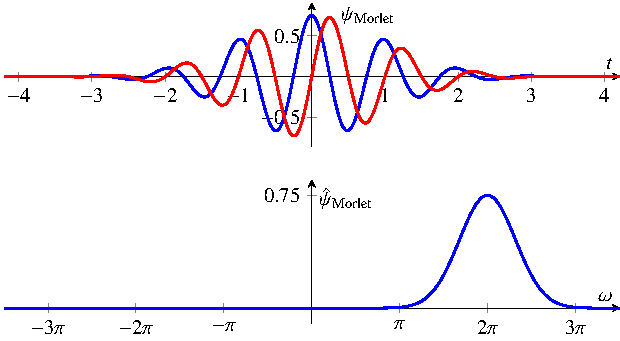
\includegraphics{papers/complex/images/morlet.pdf}
	\caption{Real- (blau) und Imaginärteil (rot) des Morlet-Wavelet für $\sigma = 2\pi$ \label{complex:morlet}}
\end{figure}

Abbildung~\ref{complex:morlet-ex} zeigt die beiden Wavelet-Transformationen unserer Beispiel-Signale.
Neu treten alle Farben auf, nicht nur jene für positive und negative Werte.
Zudem sind die Amplituden der Wavelettransformierten, also die Helligkeiten in den Bildern, nun konstant und folgen der Frequenz, statt mit dem Signal mitzuschwingen.
Ansonsten ergeben sich keine Unterschiede zu $\Wave_{\psi_\text{Gabor}}$.

\begin{figure}
	\centering
	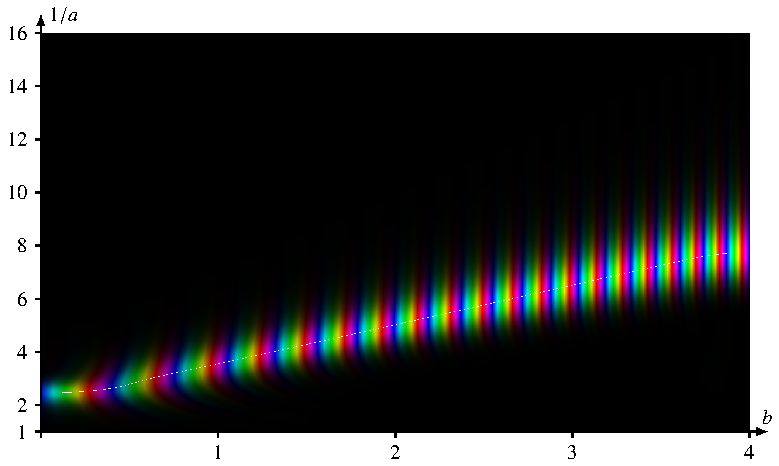
\includegraphics{papers/complex/images/chirp_morlet.pdf}
	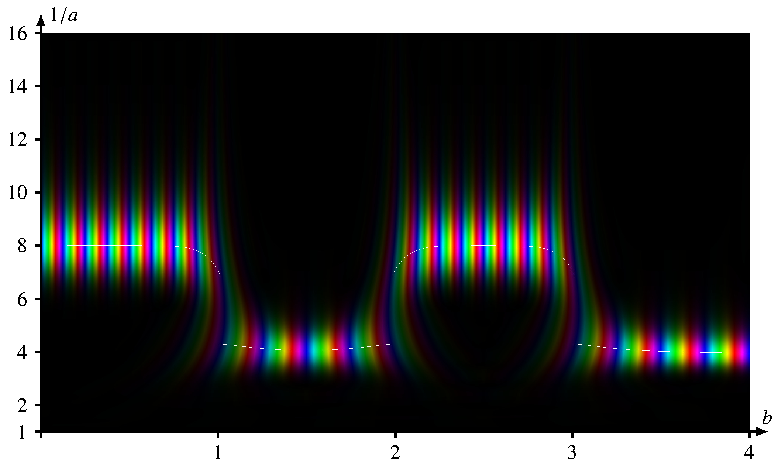
\includegraphics{papers/complex/images/square_morlet.pdf}
	\caption{Farb-codierte Wavelet-Transformationen der beiden Beispielsignale mit dem Morlet-Wavelet.}
	\label{complex:morlet-ex}
\end{figure}
